\documentclass[jou,apacite]{apa6} 
\usepackage[utf8]{inputenc}
\usepackage[spanish, es-tabla]{babel}
\usepackage{algorithm,algpseudocode}

\title{Esquemas de distribución de trabajos para un sistema ERP en la nube.}
\shorttitle{Esquemas de distribución de trabajos para un sistema ERP en la nube.}

\threeauthors{Cindy Canul\\ \texttt{110300083@ucaribe.edu.mx}}{Cristian Kumul\\ \texttt{110300097@ucaribe.edu.mx}}{Jonathan Peraza\\ \texttt{110300079@ucaribe.edu.mx}}
\threeaffiliations{Ing. Telemática\\Universidad del Caribe}{Ing. Telemática\\Universidad del Caribe}{Ing. Telemática\\Universidad del Caribe}

\date{\small{\today}}

\abstract{
	El cómputo en la nube es una tecnología prometedora como plataforma del futuro, permite crear el acceso a recursos de \textit{hardware} de manera remota. Dentro del funcionamiento de los servicios es necesario optimizar los recursos en el centro de datos por lo cual los esquemas de calendarización juegan un rol importante.
	La complejidad de la administraciónd de los recursos y la calendarización incrementa con el número de tareas, pues es un problema NP-difícil debido a las distintas características de cada \textit{host} y lo heterogéneas que son las tareas. 
}


\keywords{Cloud Computing, Scheduling}

\rightheader{Esquemas de distribución de trabajos para un sistema ERP en la nube.}
\leftheader{Esquemas de distribución de trabajos para un sistema ERP en la nube.}

\begin{document}
\maketitle    
                        
\section{Introducción}

La tecnolog\'ia en la nube ha desarrollado una infraestructura fuerte despu\'es del surgimiento del c\'omputo distribuido \cite{chen2009cloud}. Para obtener las ventajas de dicha tecnolog\'ia los usuarios simplemente necesitar\'an conectarse a internet y de esta manera tendr\'an el acceso al procesamiento de manera remota \cite{aranganathan2011aco}. Sin embargo, para aprovechar el m\'aximo potencial de \'estos recursos, es necesario tener en consideraci\'on algunas variables, ya que en un entorno en la nube existe un comportamiento din\'amico de los recursos a manera que se les provea a los usuarios el servicio \cite{shimpy2014different}.
Una de las pr\'acticas con mayor importancia en la nube es la calendarizaci\'on, ya que tiene como objetivo administrar las tareas del centro de datos para optimizar los recursos del mismo. De esta manera la eficiencia de la carga de trabajo en la nube aumenta \cite{shimpy2014different}.
En general, el objetivo de la calendarizaci\'on en la nube es utilizar los recursos de manera apropiada, mientras la carga de trabajo es distribuida uniformemente para mejorar los tiempos de ejecuci\'on \cite{shimpy2014different}.
Debido a la atenci\'on que se tiene en la tecnolog\'ia en la nube, los centros de datos han tomado un papel muy importante para los servicios empresariales \cite{shimpy2014different}. 
Un centro de datos est\'a compuesto por miles de servidores virtuales ejecut\'andose en una instancia de tiempo alojando muchas tareas, al mismo tiempo el centro de datos recibe miles de peticiones a esas tareas. Es aqu\'i en donde la programaci\'on de trabajos tiene un rol muy importante para el c\'omputo en la nube, ya que influye en el rendimiento del mismo \cite{srinivasan2014cloud}. 

El problema de la calendarizaci\'on pertenece a los algoritmos NP-Dif\'icil, lo cual tiene un amplio rango de soluciones posibles y se toma mucho m\'as tiempo de encontrar una respuesta \'optima, ya que no existe un m\'etodo para resolver estas inc\'ognitas. Sin embargo, es posible estar cerca de la mejor soluci\'on contemplando algunos entornos \cite{shimpy2014different}.

\section{Estado del Arte}

Los siguientes algoritmos de calendarizaci\'on actualmente est\'an prevaleciendo en la nube:
\begin{itemize}
	\item \textit{\textbf{Resource-Aware-Scheduling Algorithm (RASA):}} Parsa, Entezari-Maleki (2009) proponen el algoritmo \textit{RASA}, el cual utiliza las ventajas de dos algoritmos tradicionales \textit{(Max-min y Min-min)} y cubre sus desventajas. Aunque el tiempo l\'imite, la tasa de llegada, costo de ejecución y costo de comunicaci\'on no est\'an considerados \cite{parsa2009rasa}.
	
	
	\item \textit{\textbf{RSDC (Reliable Scheduling Distributed In Cloud Computing):}} Delevar, Javanmard, Shabestari y Talebi (2012) proponen un algoritmo confiable en un entorno en la nube, en este algoritmo los trabajos importantes son divididos en sub-trabajos, de tal manera que se puedan balancear las peticiones \cite{delavar2012rsdc}.
	
	
	\item \textit{\textbf{An Optimal Model for Priority based Service Scheduling Policy for Cloud Computing Environment:}} Dakshayini, Gurupased (2011), proponen un nuevo algoritmo de calendarizaci\'on que se basa en la prioridad y un esquema de control de admisi\'on. En este algoritmo, la prioridad se asigna a cada proceso admitido en la cola \cite{dakshayini2011optimal}. 
	
	
	\item \textit{\textbf{Pre-emptable Shortest Job Next Scheduling algorithm (PSJN):}}  Este algoritmo se propone en una nube privada. Utiliza la t\'ecnica de suscripci\'on preferente del algoritmo de \textit{Round Robin} junto con el siguiente proceso m\'as corto \textit{(PSN)}. Brinda beneficios de costos y mejora tiempo de respuesta y tiempo de ejecuci\'on \cite{nishant}. 
	
	
	\item \textit{\textbf{User-priority Guided Min-min scheduling algorithm:}} Se realiza una mejora para el algoritmo de balanceo de cargas, a trav\'es del algoritmo \textit{Min-min} para la calendarizaci\'on de trabajos con el fin de minimizar el tiempo de terminaci\'on del \'ultimo trabajo \textit{(makespan)} y maximizar la utilizaci\'on de los recursos \cite{chen2013user}. 
\end{itemize}

\section{Marco Teórico}

El c\'omputo en la nube es una tecnolog\'ia emergente, la cual est\'a compuesta por un grupo de recursos heterog\'eneos que proveen servicios a trav\'es de internet \cite{agarwal2014efficient}.
Esta tecnolog\'ia permite a los consumidores y negocios utilizar aplicaciones sin necesidad de instalaci\'on y con acceso a sus archivos personales en cualquier computadora con acceso a internet \cite{ahmed2012advanced}. 
El c\'omputo en la nube se puede clasificar de dos maneras:
\begin{itemize}
	\item Por la ubicaci\'on: 
	\begin{itemize}
		\item \textbf{Nube P\'ublica:} La infraestructura de c\'omputo se puede compartir entre cualquier organizaci\'on \cite{ahmed2012advanced}.
		\item \textbf{Nube Privada:} La infraestructura de c\'omputo es dedicada a una organizaci\'on en particular y no se comparte con otras organizaciones \cite{ahmed2012advanced}.
		\item \textbf{Nube H\'ibrida:} Las organizaciones pueden albergar sus aplicaciones cr\'iticas en nubes privadas y las aplicaciones con menos problemas de seguridad las puede albergar en nubes p\'ublicas \cite{ahmed2012advanced}.
	\end{itemize}
	\item Por el tipo de servicios ofrecidos: 
	\begin{itemize}
		\item \textit{\textbf{Infrastructure as a Service (IaaS):}} En \'este nivel, la infraestructura se ofrece como servicio hacia los solicitantes en forma de M\'aquinas Virtuales \textit{(VM)} \cite{agarwal2014efficient}.
		\item \textit{\textbf{Platform as a Service (PaaS):}} Es una plataforma de desarrollo de aplicaciones que se provee como servicio hacia los desarrolladores para crear aplicaciones basadas en web \cite{agarwal2014efficient}.
		\item \textit{\textbf{Software as a Service (SaaS):}} En \'este nivel el proveedor en la nube provee las aplicaciones de \textit{software} \cite{agarwal2014efficient}.
	\end{itemize}
\end{itemize}

\section{Desarrollo}

 \textit{\textbf{CloudSim}} es un nuevo, generalizado y extensible \textit{framework} de simulaci\'on, que permite el modelaje, simulaci\'on y experimentaci\'on de infraestructuras emergentes de c\'omputo en la nube y servicios de aplicaci\'on \cite{calheiros2011cloudsim}.


\renewcommand\thefigure{\arabic{figure}}
\begin{figure}[h!]
	\centering
	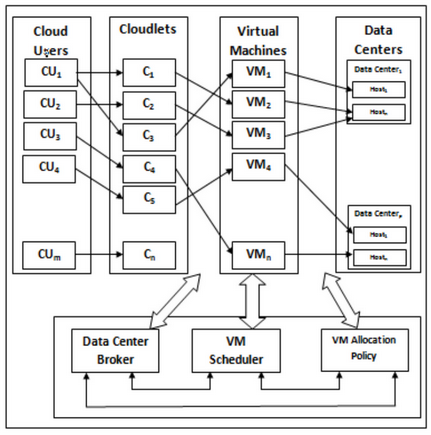
\includegraphics[scale=0.5]{media/imagenuno}
	\caption{Estilo de Trabajo de \textit{CloudSim}, Fuente: Chatterjee et al.}
	\label{fig:TrabajoCloudsim}
	
\end{figure}

Entre los componentes que proporciona dicho \textit{framework} se encuentran los siguientes:

\begin{itemize}
	\item \textit{\textbf{Cloudlet:}} Esta clase modela las aplicaciones de servicio basadas en la nube como pueden ser env\'io de contenido, redes sociales, y flujo de trabajo empresarial \cite{calheiros2011cloudsim}.
	\item \textit{ \textbf{Datacenter:}} Esta clase modela el núcleo de los servicios en un nivel de infraestructura \textit{(hardware)} que son ofrecidos por \textit{Cloud Providers (Amazon, Azure, App Engine)}. Estos son encapsulados en un conjunto de \textit{host} que pueden ser homogéneos o heterogéneos con respecto a sus configuraciones de \textit{hardware} (memoria, n\'ucleos, capacidad, y almacenamiento) \cite{calheiros2011cloudsim}.
	\item \textit{ \textbf{DatacenterBroker:}} Esta clase modela un \textit{broker}, el cual es responsable de mediar las negociaciones entre el \textit{SaaS} y los \textit{Cloud providers}; y dichas negociaciones son manejadas por los requerimientos \textit{QoS} \cite{calheiros2011cloudsim}.
	\item  \textit{\textbf{Host:}} Esta clase modela los recursos f\'isicos como una computadora o un servidor de almacenamiento \cite{calheiros2011cloudsim}.
	\item  \textit{\textbf{Vm:}} Esta clase modela una M\'aquina Virtual \textit{(VM)}, la cual es administrada y hosteada por un componente \textit{host} en la nube. Cada \textit{VM} tiene acceso a un componente que almacena las siguientes características relacionadas a una \textit{VM}: memoria accesible, procesador y tamaño de almacenamiento \cite{calheiros2011cloudsim}.
\end{itemize}

\subsection{Implementaci\'on y evaluación de los Algoritmos}

Existen varios algoritmos para calendarizar los trabajos en el c\'omputo en la nube. La mayor ventaja de estos algoritmos es obtener el mayor rendimiento. Los principales ejemplos de algoritmos de calendarizaci\'on son: \textit{FCFS, Round Robin, Min-Min, Max-Min y algoritmos de metaheurísticas}  \cite{shimpy2014different}.



De los algoritmos mencionados anteriormente, se presentan los siguientes:


\begin{itemize}
	\item \textit{\textbf{FCFS:}} Ejecuta las tareas en orden de llegada, es decir, el primero en llegar es el primero en ser atendido.
	\item \textit{\textbf{Min-Min:}} Selecciona las tareas m\'as pequeñas para ser ejecutadas primero.
	\item  \textit{\textbf{Max-Min:}} Selecciona las tareas m\'as grandes para ser ejecutadas primero.
	\item \textit{\textbf{Round Robin:}} Ejecuta las tareas en orden de llegada, si el número de tarea actual es mayor al número de máquinas virtuales reinicia el ciclo de asignación hacía la primera máquina virtual.
\end{itemize}

\subsection{Odoo - Sistema ERP \textit{OpenSource} para caso de Prueba}

Para obtener una muestra representativa del tamaño de tareas y tiempo de ejecución de las mismas, en este trabajo se hace uso de \textit{Odoo}, que es un sistema completo de gestión empresarial, de código abierto y sin costes de licencias que cubre las necesidades de las áreas de: Contabilidad y Finanzas, Ventas, RRHH, Compras, Proyectos, entre otras. \cite{odooWiki}.

\textit{Odoo} ofrece una plataforma Web, en donde se pueden administrar aplicaciones sobre gestión de recursos empresariales, además de permitir instalar aún más módulos, los cuales se pueden encontrar de manera gratuita o con algunas licencias por parte de sus desarrolladores.

\subsection{Mejorar el costo de procesamiento y el tiempo de ejecución}

El objetivo de éste proyecto es minimizar el tiempo de ejecución y el costo de procesamiento de acuerdo a los recursos heterogéneos del centro de datos. Para ello se hará la  implementación de una \textit{metaheurística} con un método llamado Optimización por Enjambre de Partículas \textit{PSO} (\textit{Particle Swarm Optimization}).\\

Optimización por Enjambre de Partículas (\textit{PSO}) es una técnica de optimización basada en la búsqueda de un óptimo global, introducida por Kennedy and Eberhart \cite{pandey2010}. 

Se eligió  \textit{PSO} debido al concepto simple que tiene \cite{poli2007},  la implementación requiere de simples operaciones matemáticas que en términos de computación no consume memoria  y la velocidad de convergencia es relativamente rápida dependiendo del número de partículas \cite{eberhart1995}.\\ 
Está claro que como toda \textit{metaheurística, PSO} no garantiza la obtención de una solución óptima en todos los casos \cite{osman2012}.

\subsection{Algoritmo \textit{PSO} y un ambiente en la nube}
\textit{PSO} permite optimizar un problema en base a una población de soluciones candidatas, que llevan el término \textit{“partículas”}, dichas partículas se mueven en un espacio de búsqueda (tienen en cuenta dos aspectos; la posición y la velocidad). Cada una realiza un movimiento influido por su mejor posición local hasta ése momento y por las mejores posiciones globales encontradas en todo el enjambre mientras recorren el espacio de búsqueda \cite{poli2007}.

Una solución potencial es representada en \textit{PSO} por un vector (partícula). Cada partícula \textit{i} tiene la misma dimensión \textit{n} y es representada de la siguiente manera \cite{pandey2010}: $X(i) = (x_{(i,1)},x_{(i,2)},...,x_{(i,n)})  $.

Para la simulación en \textit{CloudSim} éstas partículas serán las tareas en el centro de datos, $ = \{T_1 , T_2 , ... T_n\}  $.

%De igual manera las dependencias de los datos es representado por $E$,  que es, $f_j,k = (T_j,T_k) \in E$, en otras palabras $E$ es el dato producido por $T_j$ y consumido por $T_k$. 

En el centro de datos se tiene un conjunto de máquinas virtuales $VM = \{1,..,j\}$, y un conjunto de tareas $T = \{1,...,k\}$. Entonces se asume que el \textit{"promedio"} del tiempo de procesamiento de una tarea $T_k$ en la máquina virtual $VM_j$ para un tamaño de tarea conocido.
\newpage
\begin{algorithm} 
	\begin{algorithmic}[1]
		\State El número de partículas será igual al número de tareas en $ \{ t_i \} \in T $
		\State Se inicializa la posición de las partículas aleatoriamente de $VM = 1,...,j $ y con velocidad aleatoria $v_i$
		\State Para cada partícula, calcular $fitness value$.
		\State Si $fitness value$ es mejor que el anterior $pbest$, igualar $fitness value$ como el nuevo $pbest$.
		\State Seleccionar la mejor partícula como $gbest$.
		\State Para todas las partículas, calcular la velocidad y actualizar su posición.
		\State Si no se alcanza el máximo número de iteraciones, repetir el paso 3.
		
	\end{algorithmic} 
	\caption{Algoritmo PSO en la simulación}
	\label{alg:PSO}
\end{algorithm}

En el algoritmo (\ref{alg:PSO}) se muestran los pasos del PSO. Inicia con una inicialización aleatoria de la posición y velocidad de las partículas. Para la simulación, las partículas serán las tareas en el centro de datos.
El valor asignado a la dimensión de las partículas son los índices de los recursos (Máquinas Virtuales). Por lo tanto, cada tarea representa un mapeo de una tarea en todas las máquinas virtuales. Entonces la dimensión de una partícula depende del número de máquinas virtuales.
Para cada partícula se calcula un $fitnessvalue$ que es el óptimo local al nivel de partícula que se evalúa y se actualiza. 
Después se evalúa la mejor partícula como $gbest$ que sería el óptimo del enjambre.
Se delimita un número $m$, mientras no se llegue al límite la iteración continua; esto para no entrar a un ciclo que nunca termina, ya que PSO  no garantiza la obtención de una solución óptima en todos los casos \cite{osman2012}.

\section{Resultados}

\subsection{Tiempo de ejecuci\'on y costo de procesamiento}


Para evaluar los algoritmos de calendarizaci\'on seleccionados se ha implementado un entorno de c\'omputo en la nube que consiste en un \textit{datacenter}, un \textit{broker}, m\'aquinas virtuales y \textit{host}.  Con el objetivo de evaluar el tiempo de ejecuci\'on y el costo de procesamiento en el \textit{datacenter} tras ejecutar cierto n\'umero de tareas \textit{(cloudlets)}.

Para la configuraci\'on del centro de datos en \textit{CloudSim}, se utilizaron cincuenta \textit{host}, quince m\'aquinas virtuales por \textit{host} y las tareas fueron establecidas en un intervalo de 100 hasta 500 (Cuadro \ref{table:datacenter}).
Como se puede apreciar en el (Cuadro \ref{tab:host}), cada \textit{host} tuvo 20480 Mb de memoria RAM, ocho n\'ucleos de procesamiento y tienen un almacenamiento de 800 GB \'o 1 TB, estas fueron elegidas de manera aleatoria y finalmente el ancho de banda fue de 10 GB/s.

\setcounter{table}{0}
\renewcommand\thetable{\arabic{table}}
\begin{table}[h!]
	\centering
	\begin{tabular}{@{}cc@{}}
		\toprule
		\multicolumn{2}{c}{{\bf Datacenter}} \\ \midrule
		Host              & 50               \\
		VM                & 15                \\
		Cloudlet          & 100 - 500          \\ \bottomrule
		
	\end{tabular}
	\caption{Configuraci\'on \textit{Datacenter}, Fuente: Elaboraci\'on propia.}
	\label{table:datacenter}
\end{table}
 
\setcounter{table}{1}
\renewcommand\thetable{\arabic{table}}
\begin{table}[h!]
	\centering
	\begin{tabular}{@{}cc@{}}
		\toprule
		\multicolumn{2}{c}{{\bf Host}} \\ \midrule
		RAM           & 20480 MB        \\
		CPU           & 8              \\
		Storage       & 800GB - 1TB      \\ 
		BW            & 10 GB/s        
		\\ \bottomrule
	\end{tabular}
	\caption{Configuraci\'on de \textit{Host}, Fuente: Elaboraci\'on propia.}
	\label{tab:host}
\end{table}

\newpage

\setcounter{table}{2}
\renewcommand\thetable{\arabic{table}}
\begin{table}[h!]
	\centering
	\begin{tabular}{@{}cc@{}}
		\toprule
		\multicolumn{2}{c}{{\bf VirtualMachine}} \\ \midrule
		RAM               & 512 MB | 2GB          \\
		vCPU              & 2           \\
		Storage           & 10 GB                \\ 
		BW                & 1 GB/s    
		\\ \bottomrule          
	\end{tabular}
	\caption{\textit{Virtual Machine}, Fuente: Elaboraci\'on propia.}
	\label{tab:machine}
\end{table}


\setcounter{table}{3}
\renewcommand\thetable{\arabic{table}}
\begin{table}[h!]
	\centering
	\begin{tabular}{@{}cc@{}}
		\toprule
		\multicolumn{2}{c}{{\bf Cloudlet}} \\ \midrule
		length           & 100 - 1000 MI       \\
		fileSize     & 1KB - 2MB      \\
		outputSize           & 1KB - 2MB      \\ \midrule
	  
	\end{tabular}
	\caption{Configuraci\'on \textit{Cloudlet}, Fuente: Elaboraci\'on propia.}
	\label{tab:cloudlet}
\end{table}


En el Cuadro (\ref{tab:machine}) se muestran los par\'ametros que se consider\'o para las m\'aquinas virtuales, donde cada \textit{VM} tendr\'a 10 GB de almacenamiento, 512 MB  o 2 GB seleccionado de manera aleatoria, adem\'as para la caracter\'istica del procesador se tiene  la propiedad \textit{MIPS} \textit{(million instructions per second)} con 250 \'o 500 y un ancho de banda de 1 GB/s.

Para la configuraci\'on de las tareas, se tom\'o el tamaño con un intervalo de 100 MI a 1000 MI de acuerdo al tamaño mínimo y máximo en el ERP \textit{Odoo},  el par\'ametro \textit{fileSize}, que representa el tamaño del archivo de entrada, va de 1 kb a 2 mb as\'i como el archivo de salida, como par\'ametro final se tiene los \textit{outputSize} que ir\'an de 1 kb a 2 mb (Cuadro \ref{tab:cloudlet}).


\setcounter{table}{4}
\renewcommand\thetable{\arabic{table}}
\begin{table}[h!]
	\centering
	\begin{tabular}{@{}cc@{}}
		\toprule
		\multicolumn{2}{c}{{\bf Amazon EC2 t2.medium}} \\ \midrule
		vCPU     & 2     \\
		RAM &2 GB \\
		Costo por hora           & \$0.052 USD      \\ \midrule
		
	\end{tabular}
	\caption{Configuraci\'on \textit{Cloudlet}, Fuente: Elaboraci\'on propia.}
	\label{tab:cloudlet}
\end{table}

%%-----------------------------------------
%%-----------------------------------------
%%-----------------------------------------
%%-----------------------------------------
%%-----------------------------------------
%%escribir lo de la tabla aqui AMAZON y verificar texto de las tablas de arriba.
Los \textit{Cloudlets} en \textit{CloudSim} tienen un parámetro configurable que permite establecer un costo de procesamiento de manera monetaria. Para ello se consultó con el proveedor de servicios Amazon con el objetivo de  encontrar una instancia equivalente a las máquinas virtuales establecidas en la simulación. 

Se encontró que la \textit{Amazon EC2 t2.medium} cumple con las características de la simulación (Amazon,2015).

El costo de la instancia en Amazon es \$0.052 USD, entonces se configuró la característica  de los \textit{Cloudlets} con una tarifa de \$ 1.$5 e^{-5}$ USD por segundo.

\subsection{Simulación en \textit{CloudSim}}

Al tener la configuración completa del centro de datos en Cloudsim, se procedió a realizar la simulación.
Para la simulación, el programa fue ejecutado 30 veces y se ordenó ascendentemente la suma total del tiempo de ejecución de cada simulación. Se eliminaron las dos con menor tiempo y las dos con mayor tiempo, con el fin de evitar sesgos ya sea de manera positiva o negativa.

\renewcommand\thefigure{\arabic{figure}}
\begin{figure}[h!] 
	\centering
	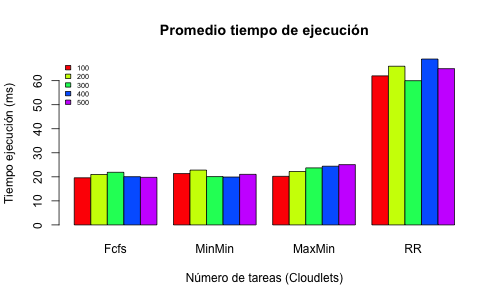
\includegraphics[scale=0.5]{media/tiempoejecucionjpg}
	\caption{Promedio tiempo de ejecuci\'on con tareas 100-500, Fuente: Elaboraci\'on propia.}
	\label{fig:tiempo}
\end{figure}



En la figura (\ref{fig:tiempo}), se puede observar el promedio del tiempo de ejecuci\'on en \emph{ms} para diferentes cantidades de tareas (de 100 a 500). A primera vista con el algoritmo \textit{FCFS} y \textit{Min-Min} se mantiene un tiempo de ejecuci\'on sin muchos cambios a pesar del aumento en la carga de tareas, a diferencia del algoritmo \textit{Max-Min} que aument\'o el tiempo de ejecuci\'on a medida que se increment\'o el n\'umero de tareas. Sin embargo para el algoritmo \textit{Round Robin} tiene el tiempo de ejecución a un poco más del doble de los anteriores. Esto es porque la tarea es procesada por diferentes máquinas virtuales.

\label{etiqueta}

\renewcommand\thefigure{\arabic{figure}}
\begin{figure}[h!] 
	\centering
	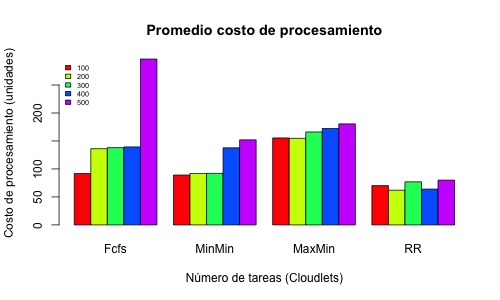
\includegraphics[scale=0.5]{media/costoproce}
	\caption{Promedio costo de procesamiento con tareas 100-500, Fuente: Elaboraci\'on propia.}
	\label{fig:costo}
\end{figure}


El costo de procesamiento, de acuerdo a cada algoritmo, se puede observar en la figura (\ref{fig:costo}), en donde el algoritmo \textit{FCFS} tiene un incremento dr\'astico al realizar la prueba con 500 tareas. El algoritmo \textit{Max-Min} se conserv\'o sin muchos cambios a pesar de la cantidad de tareas, mientras que \textit{Min-Min} tiene un menor costo de procesamiento cuando las tareas son inferiores a 300. Pero el algoritmo \textit{Round Robin} tiene un menor costo de procesamiento, ya que lo ejecutado en cada máquina virtual es la fracción de un tarea (\textit{Cloudlet}), por ende los \textit{MI} procesados son menores.
\label{etiqueta2}

\renewcommand\thefigure{\arabic{figure}}
\begin{figure}[h!] 
	\centering
	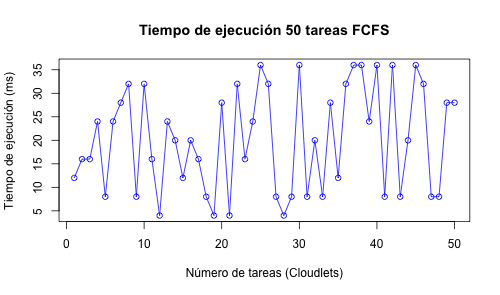
\includegraphics[scale=0.5]{media/fcfs}
	\caption{Tiempo ejecuci\'on 50 muestras \textit{FCFS}, Fuente: Elaboraci\'on propia.}
	\label{fig:ejecucion}
\end{figure}


Para mostrar el comportamiento del tiempo de ejecuci\'on por cada algoritmo, se observó una ventana de 50 muestras de una simulaci\'on de 500 tareas. En la figura (\ref{fig:ejecucion}), se puede apreciar que el algoritmo \textit{FCFS} tiene un comportamiento inestable ya que algunas tareas pueden tener menor complejidad o tamaño, lo que implica una respuesta r\'apida.

\renewcommand\thefigure{\arabic{figure}}
\begin{figure}[h!] 
	\centering
	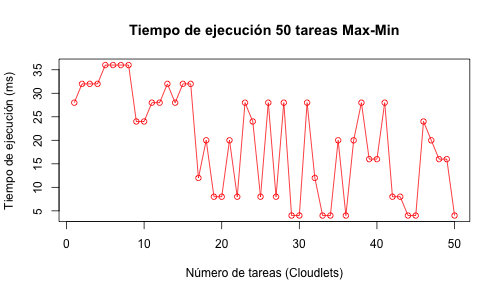
\includegraphics[scale=0.5]{media/maxmin}
	\caption{Tiempo ejecuci\'on 50 muestras \textit{Max-Min}, Fuente: Elaboraci\'on propia.}
	\label{fig:maxmin}
\end{figure}


 En la figura (\ref{fig:maxmin}) se tiene la misma simulaci\'on pero con el algoritmo \textit{Max-Min}, de acuerdo a las caracter\'isticas de este calendarizador, en las primeras tareas se toma un mayor tiempo en responder y va disminuyendo de manera gradual, sin embargo a\'un es inestable en las \'ultimas muestras ya que no se contempla el grado de complejidad, es decir el par\'ametro \textit{MI} de los \textit{cloudlets}.

 \renewcommand\thefigure{\arabic{figure}}
\begin{figure}[h!] 
	\centering
	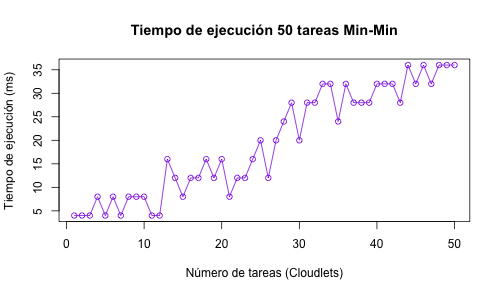
\includegraphics[scale=0.5]{media/minmin}
	\caption{Tiempo ejecuci\'on 50 muestras \textit{Min-Min}, Fuente: Elaboraci\'on propia.}
	\label{fig:minmin}
\end{figure}

En la parte de arriba se puede apreciar el algoritmo \textit{Min-Min} en el que el tiempo de ejecuci\'on fue aumentando conforme se resolv\'ian las tareas (figura \ref{fig:minmin}). Por último, en la figura (\ref{fig:roundrobin}) podemos visualizar la gráfica correspondiente al algoritmo \textit{Round Robin}. Para éste último se observan picos en el tiempo de ejecució, esto es porque la tarea es fraccionada, y para pasar al estado de \textit{COMPLETADA} cada fracción debe ser ejecutada por la máquina virtual correspondiente.


\renewcommand\thefigure{\arabic{figure}}
\begin{figure}[h!] 
	\centering
	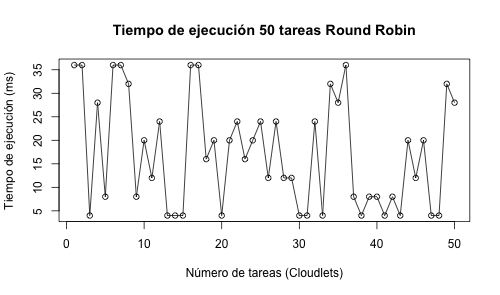
\includegraphics[scale=0.5]{media/roundrobin}
	\caption{Tiempo ejecuci\'on 50 muestras \textit{Round Robin}, Fuente: Elaboraci\'on propia.}
	\label{fig:roundrobin}
\end{figure}


\renewcommand\thetable{\arabic{table}}
\begin{table}[h!]
	\centering
	\begin{tabular}{@{}cc@{}}
		\toprule
		{\bf Algoritmo} & \multicolumn{1}{l}{{\bf Desviaci\'on est\'andar}} \\ \midrule
		FCFS & 11.00619 \\
		MAX-MIN & 8.91444 \\
		MIN-MIN & 11.25613 \\ 
		ROUND ROBIN & 11.66722 \\ \bottomrule
		
	\end{tabular}
	\caption{Desviaci\'on est\'andar del tiempo de ejecuci\'on, Fuente: Elaboraci\'on propia.}
	\label{tiempotabla}
\end{table}

Observando la desviaci\'on est\'andar de \'estas muestras anteriores, los algoritmo \textit{Min-Min}, \textit{Round Robin} y \textit{FCFS} tuvieron m\'as variaciones en las muestras con respecto a la media, mientras que el \textit{Max-Min} tuvo las variaciones por debajo de las dos anteriores (Cuadro \ref{tiempotabla}).


Por último se realizo la simulación contemplando las características de las tareas, pero sin procesamiento previo antes de calendarizar. 

Además se realizó la simulación del algoritmo propuesto en el capítulo dos. Para ello se realizaron diez simulaciones, descartando la de mejor y peor resultado.

\renewcommand\thefigure{\arabic{figure}}
\begin{figure}[h!] 
	\centering
	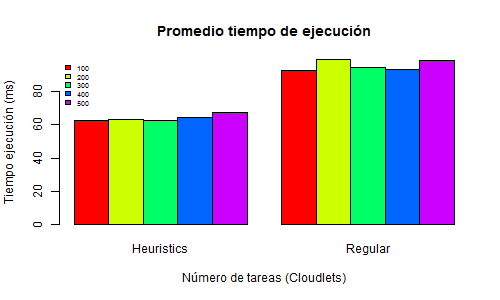
\includegraphics[scale=0.5]{media/tiempoFinal}
	\caption{Tiempo ejecuci\'on con el algoritmo propuesto(izqda.) y el tiempo de ejecución sin procesamiento previo(dcha.), Fuente: Elaboraci\'on propia.}
	\label{fig:timeF}
\end{figure}

En la figura \ref{fig:timeF} se aprecia el tiempo de ejecución del algoritmo propuesto y de la simulación sin ningún procesamiento previo. Con la heurística el promedio del tiempo de ejecución se reduce de 80 $ms$ a 60 $ms$ sin embargo es el tiempo que le lleva al centro de datos procesar esa cantidad de tareas, pero no se tiene en cuenta el tiempo previo para la búsqueda de partícula óptima. En promedio éste proceso se toma entre 20$ms$ a 30$ms$ por simulación.

\renewcommand\thefigure{\arabic{figure}}
\begin{figure}[h!] 
	\centering
	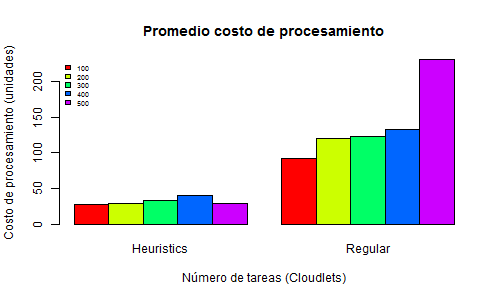
\includegraphics[scale=0.5]{media/costoFinal}
	\caption{Costo de procesamiento con el algoritmo propuesto(izqda.) y costo de procesamiento sin procesamiento previo(dcha.), Fuente: Elaboraci\'on propia.}
	\label{fig:costF}
\end{figure}

En cuanto al costo de procesamiento las simulaciones que plasmaron el resultado esperado, fue menor de 50 unidades como se muestra en la figura \ref{fig:costF}. Comparado con \textit{Round Robin} que tenia un costo de entre 60 a 80 unidades, existe una mejoría.

\section{Conclusiones}

En éste proyecto, se presentó una serie de esquemas de distribución con implementaciones sencillas para seleccionar \textit{Min-Min} y complementarlo con una metaheurística  llamada \textit{Particle Swarm Optimization (PSO)}. Se usó ésta técnica con el objetivo de minimizar el costo de procesamiento y el tiempo de ejecución en un centro de datos con un entorno en la nube. Se encontró que el esquema propuesto reduce el costo de procesamiento en 50\% en comparación con una calendarización sin procesamiento previo. Sin embargo se determinó que el mapeo de cada partícula en los recursos del centro de datos, tiene un costo en tiempo de ejecución, ya que no se observó mejoría. Por lo tanto el costo de procesamiento de una tarea en un recurso del centro de datos (en éste caso las máquinas virtuales) es inversamente proporcional al tiempo que se toma en resolver la tarea.
PSO encuentra los recursos del centro de datos en donde las tareas a procesar tendrán un menor costo. Ésta heurística tiene un carácter genérico, es decir puede ser usado para cualquier número de tareas en el centro de datos y los recursos en el centro de datos pueden tener cualquier dimensión. Ya que simplemente se incrementa el número de partículas y el espacio de búsqueda sería mayor.

\section{Trabajo a Futuro}

Como trabajo a futuro, sería interesante analizar el comportamiento del costo de procesamiento con variaciones en las políticas de alojamiento de las máquinas virtuales.

\bibliography{biblio}

\end{document}
